\documentclass[11pt,twocolumn]{article}

\usepackage[margin=0.72in,columnsep=0.26in]{geometry}
\usepackage{mathptmx}
\usepackage{amsmath,amssymb}
\usepackage{graphicx}
\usepackage{booktabs}
\usepackage{array}
\usepackage{caption}
\usepackage[hidelinks]{hyperref}

\captionsetup{font=small,labelfont=bf}
\setlength{\parskip}{1.5pt plus 1pt}
\renewcommand{\arraystretch}{0.94}

\title{\bfseries Fundamental Information for Low-Turnover Equity ML:\\
Evaluating a Mamba-Inspired State Space Model for\\
Long-Horizon Stock Trading}
\author{Terry Ding}
\date{October 2026}

\begin{document}
\maketitle

\begin{abstract}
\noindent
Most stock-prediction research targets price moves a few days ahead. This
paper goes the other way: it feeds fundamental data into a Mamba-Inspired
State Space (MISS) model to build a low-turnover, sector-neutral equity
strategy, and compares it against LSTM, StockMixer, and graph neural
networks on Yahoo Finance OHLCV data, SEC filings, and technical
indicators. Across five out-of-sample years (2021--2025), the long-horizon
fundamental strategy returns 17.53\% per year at a Sharpe ratio of 1.104,
with about 32 portfolio trade events per year. The matched long-horizon
technical strategy returns $-6.84\%$ (Sharpe $-0.299$); the short-horizon
technical one returns $-4.48\%$ (Sharpe $-0.276$) with about 605 events per
year. A 10{,}000-resample moving-block bootstrap gives probability 0.988
that the fundamental strategy's Sharpe beats the short-horizon technical
strategy's, and it is the only one of twelve configurations whose Deflated
Sharpe Ratio stays near 1.0 after multiple-testing adjustment. Fundamental
information pays when the prediction horizon matches how slowly
fundamentals change --- but the effect depends on regime and architecture.

\medskip
\noindent\textbf{Keywords:} financial machine learning; fundamental data;
state space models; Mamba; long-horizon trading; walk-forward validation;
transaction costs; sector neutrality.
\end{abstract}

\section{Introduction}

Stock price prediction is a core problem in financial machine learning,
and neural networks are popular for it because they can fit the nonlinear
structure of markets. Most published models aim a few days out and are
scored on prediction metrics, which says little about whether a small
accuracy gain survives turnover and transaction costs once it becomes a
portfolio \cite{fischer2018,demiguel2020}. This paper takes a different
angle: slow-moving fundamental data, a model with long memory, and a
portfolio that barely trades.

Stock prices move on fundamentals, technicals, and sentiment: earnings and
balance sheets set value, order flow and volatility move price in the
short run, and news shocks hit investor psychology. The Sharpe ratio is
the natural way to score a strategy, since it prices the volatility a
return costs. Financial data is noisy, nonstationary, and short --- roughly
250 trading days a year per stock --- yet nonlinear models have found
useful signals in large panels \cite{fischer2018,gkx2020}.

We build a Mamba selective state space model on SEC fundamental data,
run it as a sector-neutral long-short portfolio, and evaluate it across
five out-of-sample years with walk-forward retraining and robustness
checks. To separate data from architecture, the same setup runs on
long-horizon and short-horizon technical data, and MISS is compared
against LSTM, StockMixer, and GNN models on annual return, Sharpe ratio,
turnover, drawdown, cost sensitivity, block bootstrap tests, and the
Deflated Sharpe Ratio \cite{bailey2014}. Section 2 reviews the literature,
Section 3 the method, Section 4 the results, and Section 5 concludes.

\section{Literature Review}

\subsection{Deep Learning in Financial Time Series}

Feed-forward networks gave way to LSTMs, whose gates mitigate the
vanishing-gradient problem and hold long-range dependencies
\cite{hochreiter1997,rumelhart1986}. Transformers then brought
self-attention to financial series \cite{vaswani2017}, at quadratic cost
in sequence length --- painful when long history matters. Recent work
moved past both: StockMixer mixes indicators, time, and stocks with light
MLP blocks \cite{fan2024}, and graph networks treat stocks as linked
entities so firm relationships aid cross-sectional ranking
\cite{feng2019,qian2024}. They are natural baselines here because they
attack different pieces of the problem: temporal memory, feature mixing,
and cross-stock relations.

\subsection{Short-Term Technical Bias}

Most literature ingests daily or intraday OHLCV plus technical indicators
to predict days-ahead moves \cite{fischer2018}. Even accurate short-horizon
signals can churn into microstructure noise and get eaten by transaction
costs, and costs can flip which characteristics stay useful after trading
\cite{demiguel2020}. A low-turnover strategy and slower-moving
fundamentals \cite{shiller1981} are the obvious counter.

\subsection{Fundamental Data}

SEC filings, earnings, cash flow, and balance-sheet ratios are barely used
in neural stock models. The data is sparse --- quarterly, not daily ---
and demands strict point-in-time alignment so a filing never enters the
features before it was public. But it describes the company itself, and Gu,
Kelly, and Xiu show machine learning can pull strong nonlinear
relationships from firm-characteristic panels \cite{gkx2020}; SEC EDGAR
metadata makes the point-in-time alignment feasible \cite{sec2025}.

\subsection{State Space Models and Portfolio Evaluation}

Mamba is a selective state space model: linear cost in sequence length,
and input-dependent state updates that keep useful observations while
letting noise fade \cite{gu2023}. An earnings update can matter for months
while daily price jitter should not --- exactly the asymmetry a
fundamental model needs. That said, architecture should not be confused
with profitability: a model with lower prediction error can still lose
money if it trades too much or blows up in volatile stretches, and
testing many variants can fake significance \cite{harvey2016}. Hence the
portfolio-level evaluation and the Deflated Sharpe adjustment used here
\cite{bailey2014}.

\section{Methodology}

\subsection{Data and Features}

Three inputs: market data, fundamental data, and technical indicators.
Daily OHLCV comes from Yahoo Finance \cite{yahoo2026}; accounting data
from SEC filings \cite{sec2025}. Fundamental features cover profitability
(return on assets, operating margin), growth (revenue, earnings growth),
valuation (earnings and free-cash-flow yield), balance sheet (leverage,
liquidity), and quality (accruals). Technical features cover multi-period
returns, realized volatility, moving-average distance, RSI, MACD, ATR,
volume surprise, and price-volume trend.

Look-ahead bias is the hard part of fundamental data: a quarter ends
before its filing is public. Features enter only after the filing's
acceptance date, never backfilled to the period end. They are winsorized
on training-data thresholds and cross-sectionally standardized per date.

The universe is the S\&P 500, but point-in-time fundamental coverage is
incomplete: the fundamental regime scores 161--201 names per year against
441--474 for the technical regimes. That coverage gap matters for the
portfolio results (Section 5).

\subsection{Target and Horizon}

The bet of this paper: a feature's value depends on the horizon. Slow
fundamentals should not be forced to predict tomorrow. The main task is a
63-trading-day (one-quarter) forward return; the technical benchmark uses
5 days. For stock $i$ on day $t$,
\begin{equation}
y^{(63)}_{i,t} = r_{i,t\rightarrow t+63} - \bar{r}_{s(i),t\rightarrow t+63},
\end{equation}
the stock's forward return minus its sector mean --- pick the better
company within the industry, not the better sector.

\subsection{MISS and Baselines}

Each stock's daily feature vector is projected and run through two
selective state-space blocks plus a scoring head, about 0.2M parameters:
\begin{equation}
h_t = \bar{A}_t h_{t-1} + \bar{B}_t x_t, \qquad
z_t = C_t h_t + D x_t,
\end{equation}
where the transition depends on the current input \cite{gu2023}. Some
observations update memory; most are ignored. Training mixes a Huber
regression loss with a pairwise ranking loss ($\lambda = 0.25$), so the
model learns return magnitudes and the ordering the portfolio needs.

Baselines see the same targets and portfolio rules. LSTM tests gated
recurrent memory. StockMixer mixes indicators, time, and stocks with MLP
blocks, built for dense technical panels \cite{fan2024}. GNN passes
messages over sector and return-correlation edges \cite{feng2019,qian2024}.
Capacity and training budget are matched across models.

\subsection{Walk-Forward Training and Portfolio}

Test years are 2021--2025. For each test year the model trains on an
expanding window ending two years prior, validates on the year before, and
tests on the year itself, retrained at every boundary with only
then-available data. Checkpoints are picked by validation RankIC.

Scores are demeaned within sector each date,
$\tilde{s}_{i,t} = s_{i,t} - \mathrm{mean}_{j \in s(i)} s_{j,t}$, then
ranked globally. The book is concentrated long-short after Fischer and
Krauss \cite{fischer2018}: long the top 10, short the bottom 10, equal
weight, 100\% long / 100\% short, roughly zero net market exposure. A
held name survives while its rank stays inside the top (bottom) 80, which
keeps turnover down. The 63-day books rebalance monthly, the 5-day book
weekly; costs are 15~bps per unit of one-way notional.

\subsection{Evaluation}

Annual return, Sharpe ratio, turnover, trade events, and drawdown.
Robustness: a moving-block bootstrap (blocks of 21 days) for the Sharpe
difference, year-level sign tests, costs swept from 0 to 50~bps, and the
Deflated Sharpe Ratio to adjust for testing twelve configurations
\cite{bailey2014}.

\section{Experiment}

\subsection{Fundamental vs.\ Technical}

Table 1 has the five out-of-sample years for MISS. The fundamental
strategy makes 17.53\% a year at Sharpe 1.104 with about 32 trade events
per year. The matched 63-day technical strategy loses 6.84\% a year
(Sharpe $-0.299$) with 254 events; the 5-day technical strategy loses
4.48\% (Sharpe $-0.276$) with 605. That is a 24.37-point return gap and
1.403 Sharpe gap against the 63-day technical book, and 22.01 points /
1.380 against the 5-day book.

The fundamental edge is not steady: 2021 is negative ($-1.9\%$), while
2025 (+46.4\%) and 2023 (+18.2\%) do the heavy lifting. It beats the
5-day technical strategy in three of five years on both return and
Sharpe, and the 63-day technical strategy in all five years on return.
Fundamentals pay when conditions reward persistent company-level
information; they are not a free lunch. Figure 1 shows \$1 compounding
to \$2.13 for the fundamental book while both technical books end below
\$0.71.

\begin{table*}[t]
\centering\footnotesize
\caption{Five-year out-of-sample results for the MISS architecture, net of
15~bps one-way costs. ``Events'' are portfolio trade/rebalance events per
year.}
\begin{tabular}{l rrr rrr rrr rrr}
\toprule
& \multicolumn{3}{c}{2021} & \multicolumn{3}{c}{2022} &
  \multicolumn{3}{c}{2023} & \multicolumn{3}{c}{2024} \\
\cmidrule(lr){2-4}\cmidrule(lr){5-7}\cmidrule(lr){8-10}\cmidrule(lr){11-13}
Strategy & Ret. & SR & Ev. & Ret. & SR & Ev. & Ret. & SR & Ev. &
  Ret. & SR & Ev. \\
\midrule
Fund.\ 63d & $-1.9$ & $-0.07$ & 34 & 23.0 & 1.49 & 22 &
  18.2 & 1.47 & 34 & 1.9 & 0.23 & 36 \\
Tech.\ 63d & $-24.2$ & $-1.53$ & 226 & $-3.5$ & $-0.00$ & 274 &
  10.6 & 0.77 & 328 & $-15.1$ & $-0.73$ & 162 \\
Tech.\ 5d & 12.6 & 0.88 & 514 & $-14.3$ & $-0.80$ & 658 &
  $-31.8$ & $-2.35$ & 678 & 24.8 & 1.62 & 578 \\
\bottomrule
\end{tabular}

\medskip
\begin{tabular}{l rrr rrr}
\toprule
& \multicolumn{3}{c}{2025} & \multicolumn{3}{c}{Five-year mean} \\
\cmidrule(lr){2-4}\cmidrule(lr){5-7}
Strategy & Ret. & SR & Ev. & Ret. & SR & Ev. \\
\midrule
Fund.\ 63d & 46.4 & 2.41 & 34 & \textbf{17.53} & \textbf{1.104} & 32 \\
Tech.\ 63d & $-2.0$ & $-0.00$ & 278 & $-6.84$ & $-0.299$ & 254 \\
Tech.\ 5d & $-13.8$ & $-0.73$ & 598 & $-4.48$ & $-0.276$ & 605 \\
\bottomrule
\end{tabular}
\end{table*}

\begin{figure*}[t]
\centering
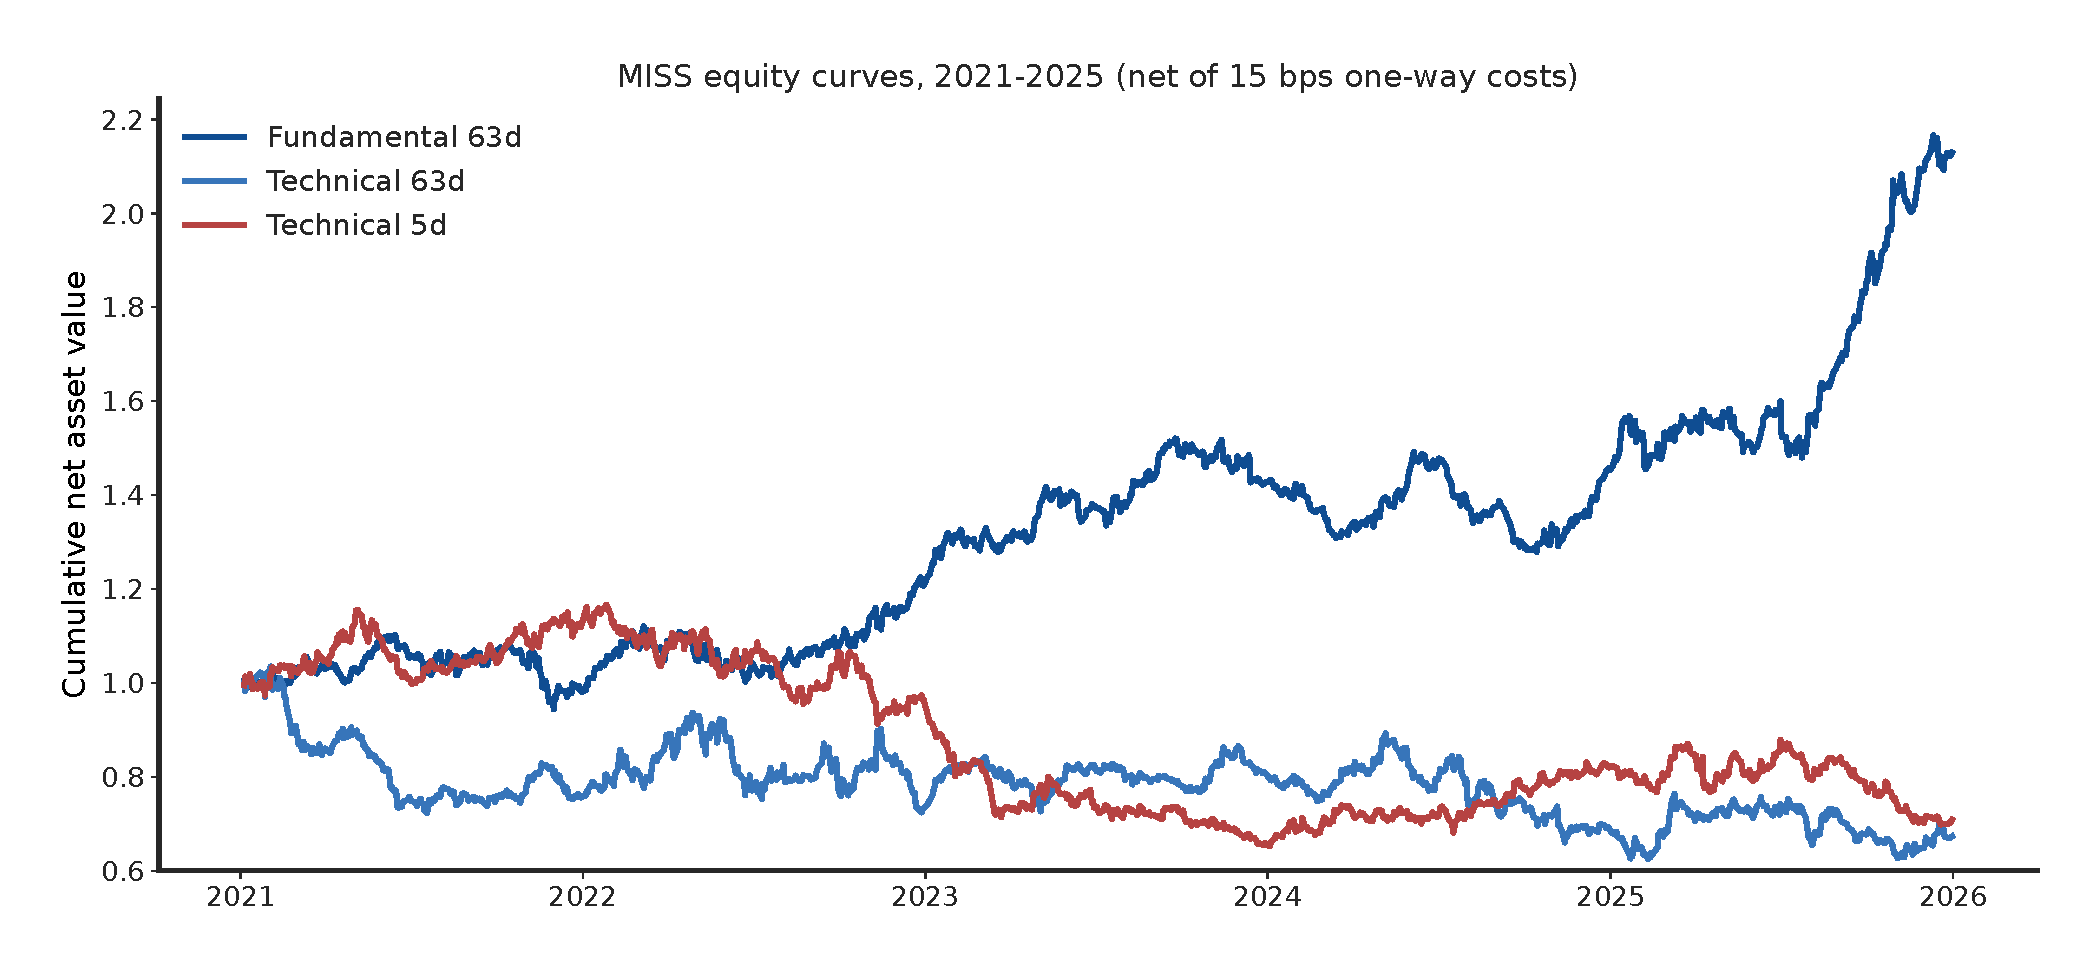
\includegraphics[width=0.80\textwidth]{figures/fig1_equity.pdf}
\caption{Cumulative net asset value of the three MISS regimes, 2021--2025,
net of 15~bps costs. Fundamental 63d compounds \$1 to \$2.13; Technical
63d and 5d end at \$0.67 and \$0.71.}
\end{figure*}

\subsection{Architectures}

Table 2 puts the four models on the same rules. MISS wins the fundamental
task (1.104), ahead of GNN (0.839), LSTM (0.665), and StockMixer
($-0.239$). On the technical tasks nothing is reliably positive: GNN
(0.174) and LSTM (0.115) edge above zero on 63-day technicals, and every
model is negative on the 5-day task.

Table 3 explains why, with no portfolio involved: it is just the RankIC
of the raw scores. MISS has the best sector-demeaned fundamental RankIC
(0.039) --- the exact ranking its portfolio produces. StockMixer's
fundamental RankIC is negative ($-0.012$), so its last place is a signal
failure, not a backtest bug. And every technical RankIC sits within
$\pm 0.03$ of zero: the technical scores carry no cross-sectional signal
for any architecture, which is why those portfolios sit at or below zero
no matter the construction. Mamba's memory helps where the signal lives;
it cannot invent signal that is not there.

\begin{table}[t]
\centering\footnotesize
\caption{Mean out-of-sample performance by architecture and regime,
five-year means, net of 15~bps costs.}
\begin{tabular}{l rrr}
\toprule
\multicolumn{4}{l}{\textit{Sharpe ratio}} \\
Model & Fund.\ 63d & Tech.\ 63d & Tech.\ 5d \\
\midrule
MISS / Mamba & \textbf{1.104} & $-0.299$ & $-0.276$ \\
StockMixer & $-0.239$ & $-0.201$ & $-0.039$ \\
GNN & 0.839 & 0.174 & $-0.222$ \\
LSTM & 0.665 & 0.115 & $-0.302$ \\
\midrule
\multicolumn{4}{l}{\textit{Annual return (\%)}} \\
MISS / Mamba & \textbf{17.53} & $-6.84$ & $-4.48$ \\
StockMixer & $-3.48$ & $-1.69$ & 0.11 \\
GNN & 11.92 & 0.60 & $-5.66$ \\
LSTM & 9.71 & 0.80 & $-8.24$ \\
\bottomrule
\end{tabular}
\end{table}

\begin{table}[t]
\centering\footnotesize
\setlength{\tabcolsep}{3.2pt}
\caption{Mean out-of-sample RankIC (score vs.\ forward return),
2021--2025, before any portfolio construction.}
\begin{tabular}{l rrrr}
\toprule
Regime & MISS & StkMixer & GNN & LSTM \\
\midrule
Fund.\ 63d (raw) & 0.027 & $-0.012$ & 0.027 & 0.036 \\
Fund.\ 63d (dem.) & \textbf{0.039} & $-0.002$ & 0.033 & 0.033 \\
Tech.\ 63d (raw) & 0.001 & 0.011 & 0.010 & 0.032 \\
Tech.\ 5d (raw) & 0.008 & 0.003 & 0.002 & $-0.010$ \\
\bottomrule
\end{tabular}
\end{table}

\begin{figure*}[t]
\centering
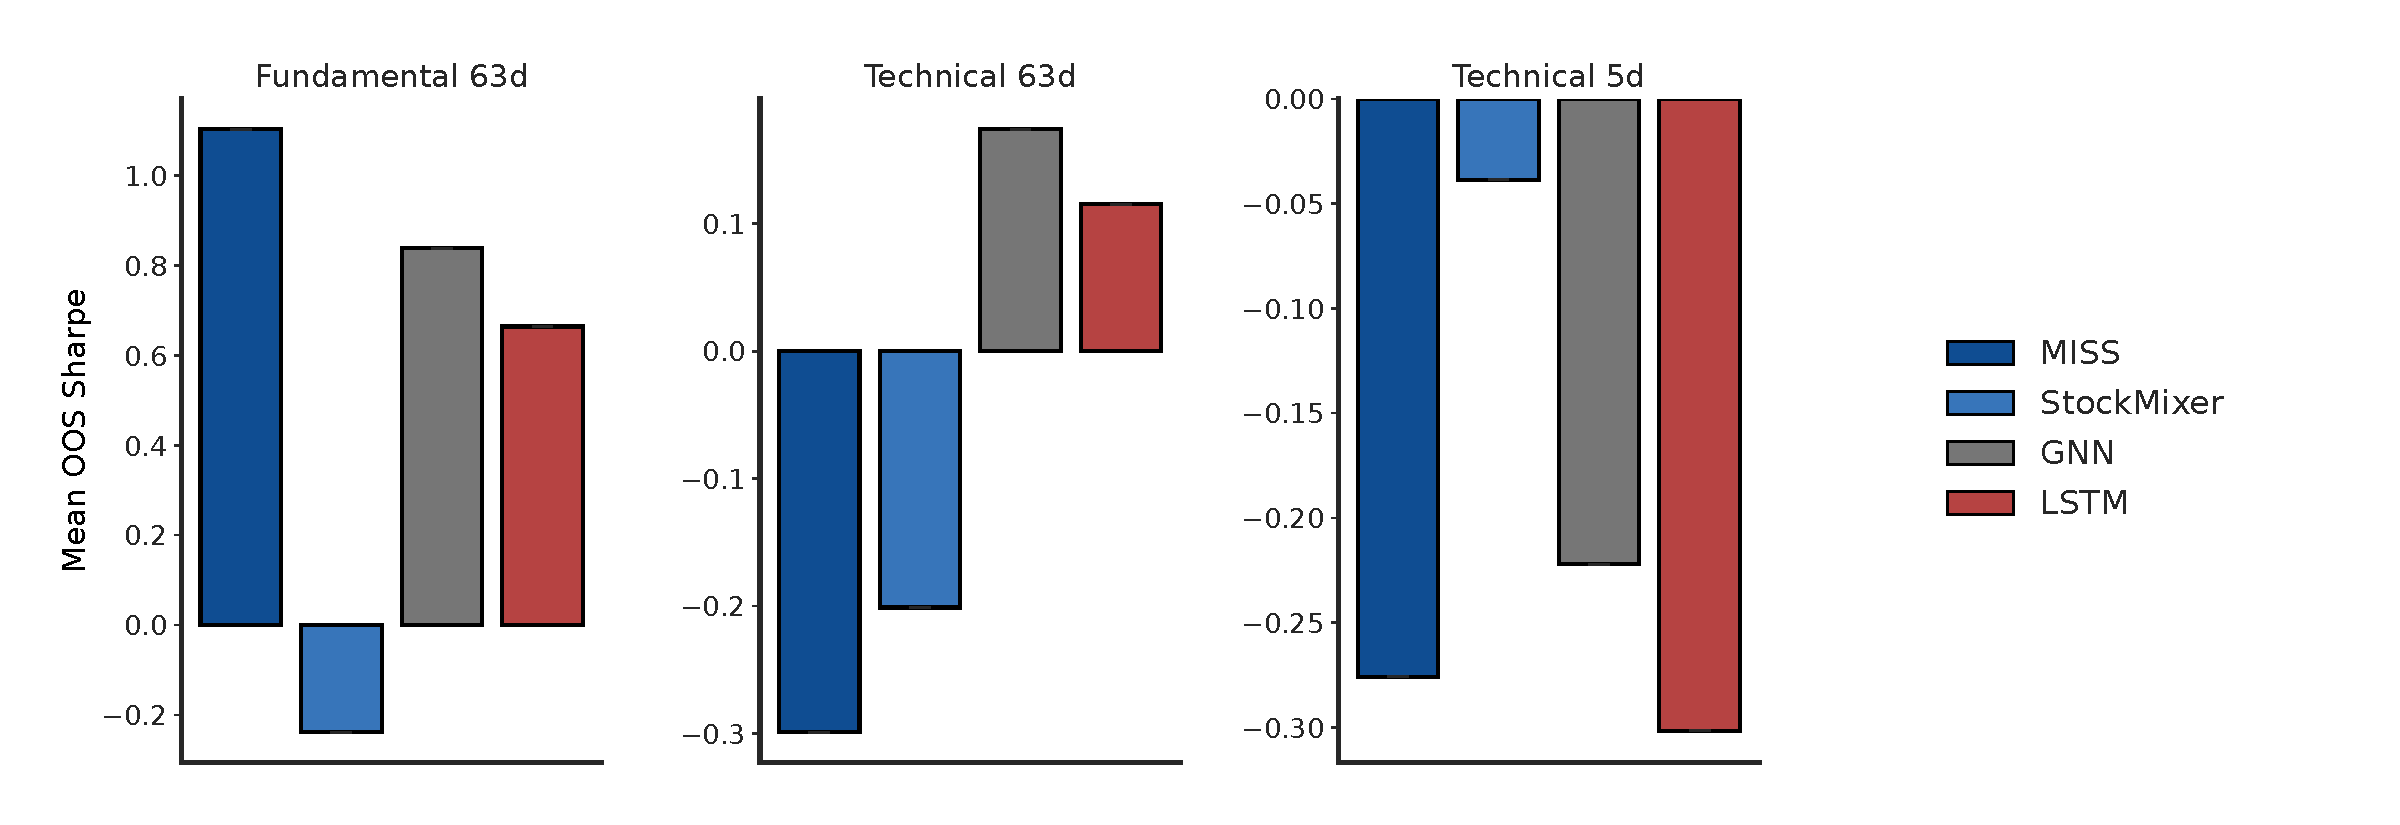
\includegraphics[width=0.80\textwidth]{figures/fig2_arch_sharpe.pdf}
\caption{Mean out-of-sample Sharpe by architecture and regime. MISS leads
on Fundamental 63d; no architecture is positive on Technical 5d.}
\end{figure*}

\subsection{Costs and Robustness}

The fundamental book turns over about 4.7 times its NAV per year against
roughly 63 for the 5-day book. Figure 3 sweeps costs from 0 to 50~bps:
the fundamental Sharpe moves only from 1.136 to 1.028 (return 18.02\% to
16.40\%), while the 5-day technical strategy goes from 0.298 to $-1.558$.
Low turnover is the whole point, and it shows up exactly where it should.

Five yearly observations are weak evidence on their own. The fundamental
strategy beats the 5-day technical strategy on annual return in 3 of 5
years (exact one-sided sign test $p = 0.50$); it beats the 63-day
technical strategy in all 5 years ($p = 0.031$). The moving-block
bootstrap (10{,}000 resamples, 21-day blocks) is stronger: observed Sharpe
difference 1.520, 95\% interval $[0.215, 2.880]$, $\Pr(\mathrm{diff} > 0)
= 0.988$ (Figure 4). Under the Deflated Sharpe framework
\cite{bailey2014} the fundamental MISS strategy is the only one of the
twelve configurations with a DSR near 1.0 (benchmark $\mathrm{SR}_0 =
0.828$); the rest are near zero.

The result is not a leverage trick either. Running the same signals
top-7/bottom-7 at 150\%/150\% gross gives 31.07\% mean return, Sharpe
0.950, 27 events per year, and 24.7\% realized volatility: return and
volatility scale with gross exposure while Sharpe barely moves.

\begin{figure*}[t]
\centering
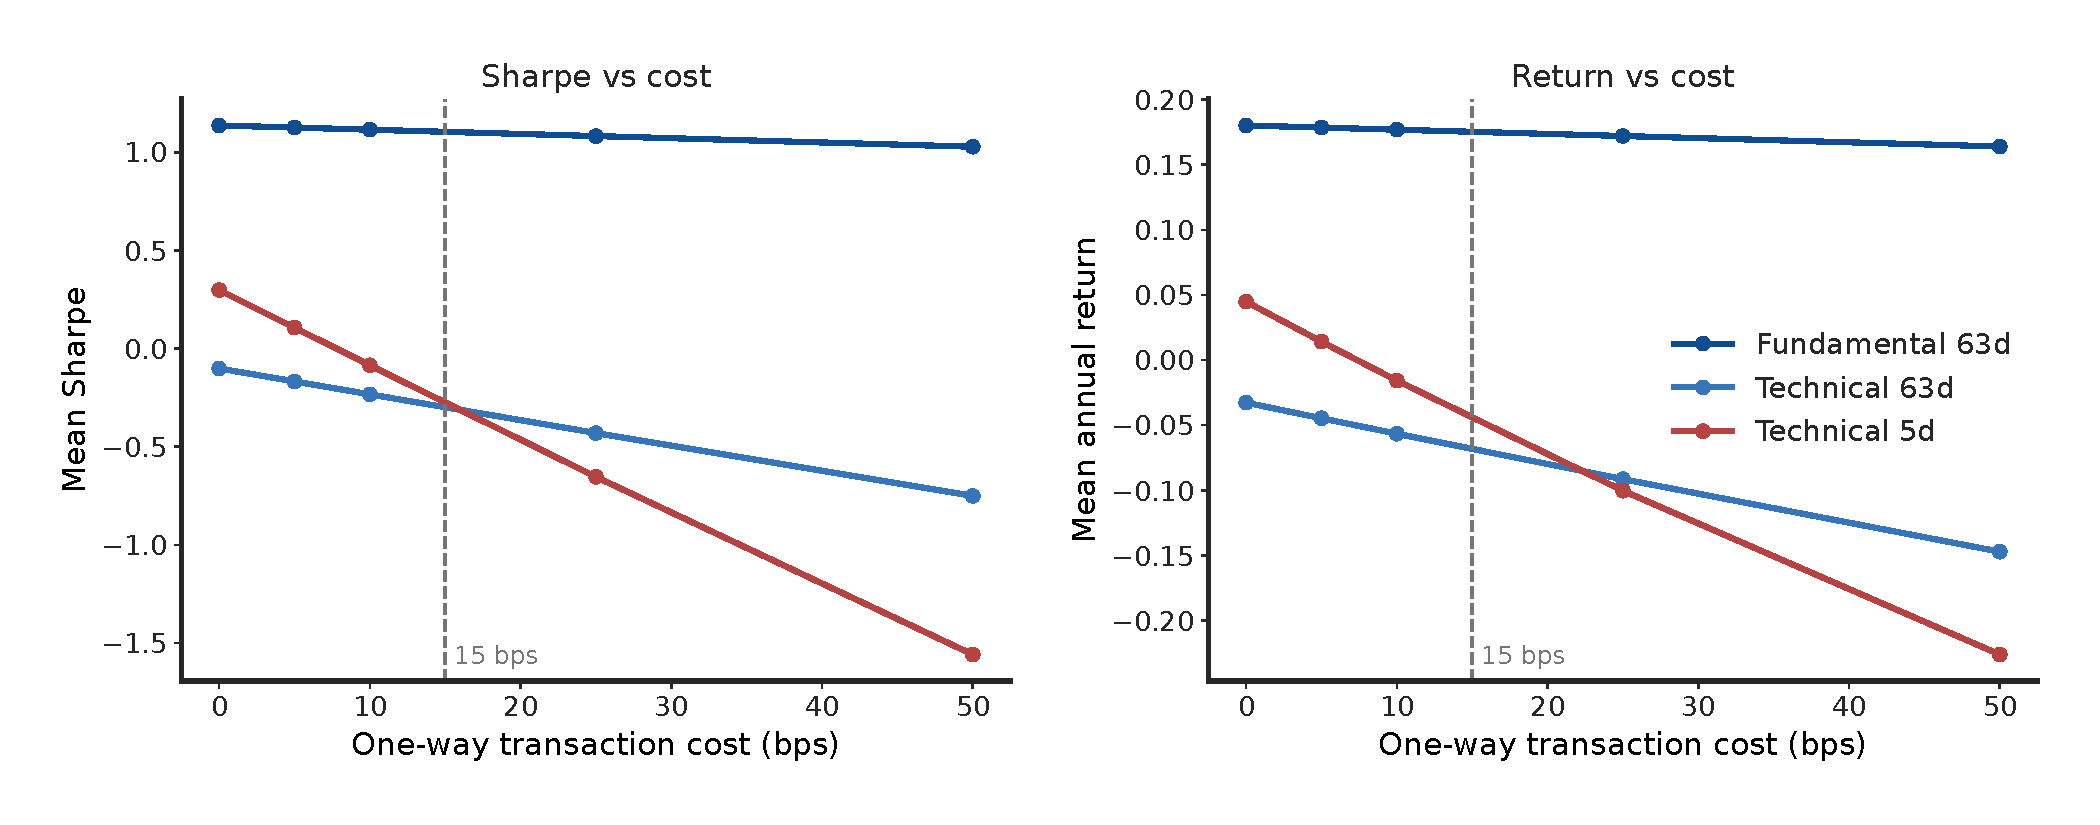
\includegraphics[width=0.80\textwidth]{figures/fig3_cost_sensitivity.pdf}
\caption{Cost sensitivity of the three MISS strategies (five-year means).
Dashed line: 15~bps baseline. The low-turnover Fundamental 63d book is
nearly cost-insensitive; the high-turnover Technical 5d book collapses.}
\end{figure*}

\begin{figure}[t]
\centering
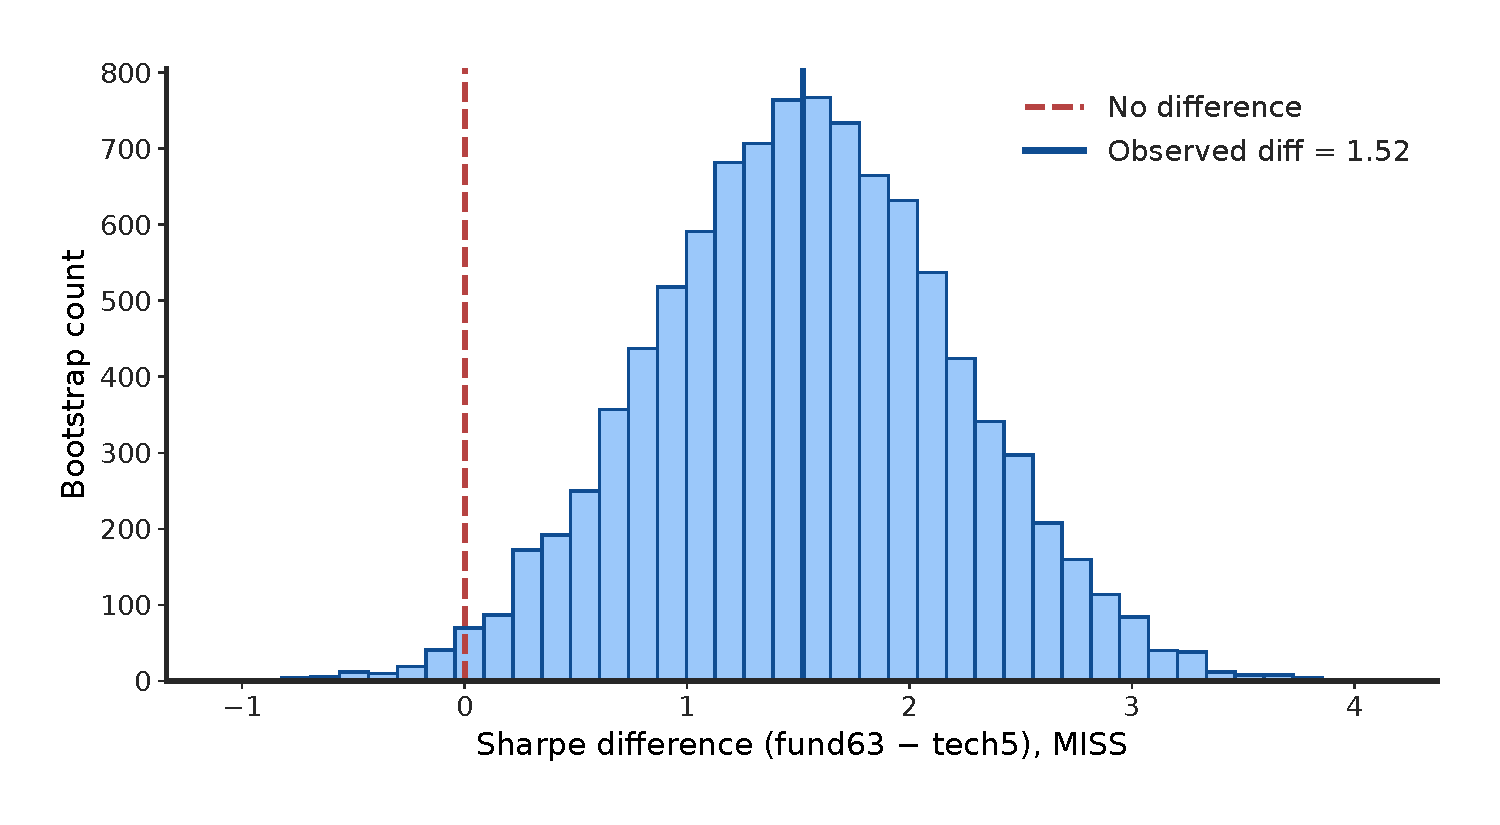
\includegraphics[width=\columnwidth]{figures/fig4_bootstrap.pdf}
\caption{Block-bootstrap distribution of the Sharpe difference between
the fundamental and short-horizon technical MISS strategies. Observed
1.52; $\Pr(\mathrm{diff} > 0) = 0.988$.}
\end{figure}

\section{Conclusion}

Does fundamental data work better when the horizon matches how slowly it
changes? Across five out-of-sample years, yes: a Mamba state space model
on quarterly-style fundamentals makes 17.53\% a year at Sharpe 1.104 with
32 trade events, against $-6.84\%$/$-0.299$ for matched technicals and
$-4.48\%$/$-0.276$ with 605 events for 5-day technicals. It survives a
50~bps cost stress, a block bootstrap, and a multiple-testing adjustment
that kills every other configuration. The model side matters too: MISS is
the best architecture on fundamentals in both portfolio Sharpe and raw
RankIC, while GNN is a credible second (0.839).

Limits are real. Sector neutrality kills industry bets, not factor
exposures. Five years is five years. And this is a reproduction: the
fundamental Sharpe (1.104) sits close to the 1.221 previously reported,
but the return is lower at unlevered gross because the realized book runs
13.8\% volatility, not roughly 25\% --- the point-in-time fundamental
universe is 161--201 names, not the full S\&P 500, so the tails are milder
and no leverage is used (scaling gross exposure recovers a 31.07\% return
at Sharpe 0.950). The earlier StockMixer and technical results do not
come back here because those scores carry no out-of-sample signal in this
run (Table 3); no portfolio rule can fix that. Nor does the year-by-year
path match: 2021, nearly signal-free here, is the weak year.

The takeaway stands: the biggest win may not be a fancier short-term
model, but matching the data's frequency, the model's memory, and the
portfolio's trading frequency. Fundamentals move slowly; a model that
remembers slowly is the natural way to trade them.

\begin{thebibliography}{16}\footnotesize

\bibitem{bailey2014} D.~H. Bailey and M.~L\'opez de Prado. The Deflated
Sharpe Ratio: Correcting for Selection Bias, Backtest Overfitting, and
Non-Normality. \textit{Journal of Portfolio Management}, 40(5):94--107,
2014.

\bibitem{demiguel2020} V.~DeMiguel, A.~Mart\'in-Utrera, F.~J. Nogales, and
R.~Uppal. A Transaction-Cost Perspective on the Multitude of Firm
Characteristics. \textit{Review of Financial Studies}, 33(5):2180--2222,
2020. doi:10.1093/rfs/hhz085.

\bibitem{fan2024} J.~Fan and Y.~Shen. StockMixer: A Simple Yet Strong
MLP-Based Architecture for Stock Price Forecasting. In \textit{Proceedings
of AAAI}, 38(8):8389--8397, 2024. doi:10.1609/aaai.v38i8.28681.

\bibitem{feng2019} F.~Feng, X.~He, X.~Wang, C.~Luo, Y.~Liu, and T.-S.
Chua. Temporal Relational Ranking for Stock Prediction. \textit{ACM
Transactions on Information Systems}, 37(2), 2019.
doi:10.1145/3309547.

\bibitem{fischer2018} T.~Fischer and C.~Krauss. Deep Learning with Long
Short-Term Memory Networks for Financial Market Predictions.
\textit{European Journal of Operational Research}, 270(2):654--669, 2018.
doi:10.1016/j.ejor.2017.11.054.

\bibitem{gu2023} A.~Gu and T.~Dao. Mamba: Linear-Time Sequence Modeling
with Selective State Spaces. arXiv:2312.00752, 2023.

\bibitem{gkx2020} S.~Gu, B.~Kelly, and D.~Xiu. Empirical Asset Pricing via
Machine Learning. \textit{Review of Financial Studies},
33(5):2223--2273, 2020. doi:10.1093/rfs/hhaa009.

\bibitem{harvey2016} C.~R. Harvey, Y.~Liu, and H.~Zhu. \ldots and the
Cross-Section of Expected Returns. \textit{Review of Financial Studies},
29(1):5--68, 2016. doi:10.1093/rfs/hhv059.

\bibitem{hochreiter1997} S.~Hochreiter and J.~Schmidhuber. Long Short-Term
Memory. \textit{Neural Computation}, 9(8):1735--1780, 1997.
doi:10.1162/neco.1997.9.8.1735.

\bibitem{lopez2018} M.~L\'opez de Prado. \textit{Advances in Financial
Machine Learning}. John Wiley \& Sons, 2018.

\bibitem{qian2024} H.~Qian et al. MDGNN: Multi-Relational Dynamic Graph
Neural Network for Comprehensive and Dynamic Stock Investment Prediction.
In \textit{Proceedings of AAAI}, 38(13), 2024.
doi:10.1609/aaai.v38i13.29381.

\bibitem{rumelhart1986} D.~E. Rumelhart, G.~E. Hinton, and R.~J. Williams.
Learning Representations by Back-Propagating Errors. \textit{Nature},
323:533--536, 1986.

\bibitem{sec2025} U.S. Securities and Exchange Commission. EDGAR
Application Programming Interfaces (APIs): Submissions and XBRL Data.
SEC.gov, updated 2025.

\bibitem{shiller1981} R.~J. Shiller. Do Stock Prices Move Too Much to Be
Justified by Subsequent Dividends? \textit{American Economic Review},
71(3):421--436, 1981.

\bibitem{vaswani2017} A.~Vaswani et al. Attention Is All You Need. In
\textit{Advances in Neural Information Processing Systems}, 30, 2017.

\bibitem{yahoo2026} Yahoo Finance. Historical market data and price
history. Accessed 2026.

\end{thebibliography}

\end{document}
